\section{Hybrid Model}\label{hybrid-model}

\subsection{Overview}

Nomenclature\\
\begin{tabular}{ll}
$Q_{int}$ & Internal heat gain\\
$h_s$ & Convective heat transfer coefficient\\
$A_s$ & Zone surface area\\
$T_s$ & Zone surface temperature\\
$T_z$ & Zone air temperature\\
$T_{iz}$ & Interzone air temperature\\
$T_o$ & Outdoor air temperature\\
$T_{sup}$ & Air system supply air temperature\\
$q_{inf}$ & Infiltration air flow rate\\
$\dot{m}_i$z & Interzone air mass flow rate\\
$\dot{m}_{sys}$ & Air system mass flow rate\\
$V$ & Zone volume\\
$\rho_{air}$ & Air density\\
$C_z$ & Heat capacity of zone air and internal thermal mass\\
$C_p$ & Zone air specific heat\\
$C_T$ & Heat capacity multiplier\\
\end{tabular}

The hybrid modeling combines forward and inverse physics-based modeling taking advantage of measured zone air temperature data to perform targeted calibration on specific inputs. The hybrid modeling approach aims to enhance the current energy retrofit practices not only offering more user-friendly energy modeling environments but also providing more accurate estimates of energy savings at the same time. The hybrid model avoids input parameters that are hard to measure and replace them to easily measurable data, which integrates physics-based and data-driven modeling methods. Parameters such as interior thermal mass and air infiltration rates are required in physics-based models, and they have significant impacts as they are driving factors for the dynamic performance of buildings. An accurate estimate of interior thermal mass has been a difficult problem because the building usually has various amounts of furniture and changeable partitions. The air infiltration rate changes in time and dynamically interacts with indoor and outdoor climatic conditions. However the accurate estimation of the data is almost impossible to collect without a fan pressurized test, which can not be easily done by typical energy modelers (Gowri et al. 2009). The hybrid model introduces an approach that represents the interior thermal mass in EnergyPlus, one with traditional interior mass object and the other with capacitance multiplier approach. Also the approach presents fundamentals of the infiltration modeling in energy simulation and provides mathematical derivation of the hybrid model. 

\subsection{Hybrid modeling approaches}\label{hybrid-modeling-approaches}

Solving building energy and environmental problems inversely using measured data gets more attention as more data are easily and freely available. (Yinping Zhang et al. 2015). Measurements are to supplement to reduce discrepancies or to identify model parameters, nevertheless the majority of efforts go into the derivation of the dynamic inverse modeling. Inverse modeling is a discipline that applies mathematical techniques to combine measurements and models. Inverse modeling can provide solutions when direct measurements of model parameters are not widely available, rendering the use of numerical techniques.

The new hybrid modeling approach uses the inverse modeling method to improve the accuracy of the building energy simulation for existing buildings, which adds measured data to solve uncertain model parameters. The hybrid modeling approach builds upon the virtue of the physics-based model taking advantage of measured data. The approach uses measured zone air temperature to replace highly uncertain parameters such as internal thermal mass and infiltration airflow rate in the zone heat balance calculations by solving the reformulated zone heat balance equations. Figure~\ref{fig:hybrid-model-conceptual-diagram} illustrates a conceptual diagram that easily express the concept of the hybrid modeling approach. 

\begin{figure}[h]
\begin{center}
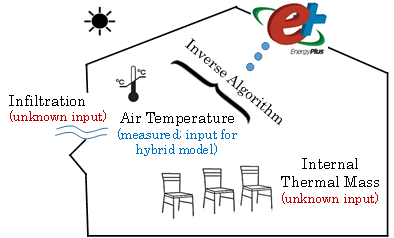
\includegraphics[width=295pt]{media/img_HybridModel-1.png}
\caption{Hybrid model conceptual diagram}\protect \label{fig:hybrid-model-conceptual-diagram}
\end{center}
\end{figure}

Temperature data are easily available nowadays and are used for controls of indoor environments due to a wider use of low-cost thermostats with data loggers. Thermal mass plays an important role in energy modeling in predicting the transient cooling or heating loads and in strategizing heating, ventilation, and air conditioning (HVAC) system controls. There has been numerous research on energy efficient design and reducing peak cooling demand using thermal mass  (Balaras 1996; Xu \& Zagreus 2010; Karlsson 2012; Building \& Simulation n.d.; Ma \& Guo 2015). Building envelop takes a significant amount of thermal mass. Physical details of envelop model parameters such as density, volume, and specific heat capacity can be easily determined per construction documents. However the internal thermal mass has not been well highlighted in most of building energy simulation practices. Components such as furniture, partitions have mass with mass with thermal capacitance cannot ignorable in the thermal heat transfer models. Although internal thermal mass has a substantial influence in prediction of cooling or heating requirements, it is very difficult to obtain detailed physical properties required for inputs in the current simulation tools (Zeng et al. 2011; Wang \& Xu 2006). This is one key factor leading to high uncertainty for energy performance analysis and simulations results.

There have been research efforts in exploring ways to estimate the thermal mass of zones. Braun et al provided thermal mass control strategies, including interior thermal mass estimates that optimize the heating and cooling energy cost savings (Lee \& Braun 2008; Braun \& Chaturvedi 2002). Their studies develop a simplified heat balance equation, and derived the inverse model, using short term measured data to identify control strategies shifting and reducing peak cooling loads. It provides background on the concept and the problem of optimizing zone temperature set-points. Wang et al provided a method to estimate the building interior thermal mass, using a thermal network structure of lumped thermal masses and operational data to estimate the lumped parameters (Wang \& Xu 2006). A genetic algorithm was used to estimate the lumped interior thermal parameters. The DOE reference model (Deru et al. 2011) includes representative typical inputs for interior mass with assumptions of standard wood, medium smooth interior furnishing conditions, which helps understand the significance of the interior mass in the energy models. These approaches have limitations such as requiring longer hours of data and additional input data in their custom energy models, which burden the use in general cases.

The hybrid modeling approach can overcome the problem, which does not require the input of interior thermal mass in energy simulations. The study explores an approach that derives physical characteristics of the interior thermal mass. The approach solves the zone heat balance equation using measured zone air temperature (an input to the hybrid model) without the need of traditional input of zone interior thermal mass (an output of the hybrid model). The zone interior thermal mass in the hybrid modeling is represented as a temperature capacitance multiplier for the zone air thermal mass. The capacitance multiplier is calculated based on the input of zone air temperature and all other traditional inputs to energy models. The calculated capacitance multiplier is then used in normal energy modeling and simulation to calculate cooling and heating loads and energy use in buildings. It should be noted that the derived algorithms are generic and can be adopted by other building energy modeling tools. The study uses EnergyPlus to demonstrate the approach. The paper provides technical details to derive algorithms for estimation of the interior thermal mass, validation, implementation in EnergyPlus, and verification of the simulation results.

\subsection{Zone air heat balance algorithm}\label{Zone-air-heat-balance-algorithm}

The hybrid model algorithms are built upon the physics-based zone heat balance equation reformulated to solve a partially inverse problem. The approach inverses the physics-based energy model, reformulating the heat balance algorithm with measured zone air temperature data (traditionally results/output of the physics-based model) to solve highly unknown parameters for internal thermal mass and infiltration air flow rates (traditionally input of the physics-based model).

EnergyPlus provides algorithms to solve the zone air energy balance equation that uses the analytical solution to calculate the derivative term respect to time. The basis for the zone air system integration is to formulate energy balances for the zone air as shown in following equations and solve the resulting ordinary differential equations. 

\begin{equation}
C_z \frac {dT_z} {dt} = \Sigma Q_i +\Sigma[h_i A_i (T_{si} - T_z)] + \Sigma [\dot{m}_i C_p (T_{zi}-T_z)] + \dot{m}_{inf} C_p (T_o - T_z) + Q_{sys}
\end{equation}
\begin{equation}
C_z = V \rho_{air} C_p C_T
\end{equation}

The sum of zone loads and the provided air system energy equals the change in energy stored in the zone. Typically the zone capacitance, $C_z$ includes the zone air only when formulating energy balances for the zone air. The internal thermal mass, including furniture, books, and changeable partitions, is assumed to be in thermal equilibrium with the zone air, thus it is added in the zone heat capacitance, $C_z$.  The infiltration airflow rate, $q_inf$ changes for different conditions depending on outdoor temperature, wind speed, and HVAC system operations. The energy provided from systems to the zone is represented as $Q_{sys}$.

EnergyPlus provides heat balance solution algorithms of 3rd order backward difference and analytical solution to solve the zone air energy balance equation. The 3rd order finite difference approximation provides stability without requiring a prohibitively small time step, the method still has truncation errors and requires a fixed time step length for the previous three simulation time steps. Therefore, different time step lengths for the previous three simulation time steps may make the temperature coefficients invalid. The analytical solution algorithm is an integration approach that provides a possible way to obtain solutions without truncation errors and independent of time step length and only requires the zone air temperature for one previous time step. The hybrid modeling approach uses the analytical solution for internal thermal mass inverse calculation and the 3rd order backward difference for infiltration inverse calculation. 


\subsection{Internal thermal mass hybrid modeling method}\label{internal-thermal-mass-hybrid-modeling method}

There are two approaches to model internal thermal mass in EnergyPlus. One approach is to use the internal mass objects to define construction specifications of internal furnishing materials, and the other is to use the temperature capacitance multipliers. The multiplier increases zone air capacity as it represents the effective storage capacity of the zone interior thermal mass. Figure~\ref {fig:two-approaches-of-representing-interior-thermal-mass-in-EnergyPlus} illustrates two approaches of representing interior thermal mass in EnergyPlus.

\begin{figure}[h]
\begin{center}
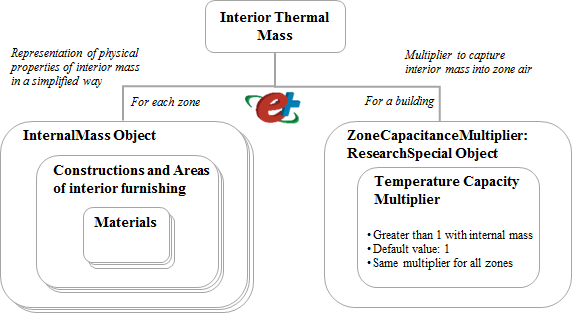
\includegraphics[width=428pt]{media/img_HybridModel-2.png}
\caption{Two approaches of representing interior thermal mass in EnergyPlus}\protect \label{fig:two-approaches-of-representing-interior-thermal-mass-in-EnergyPlus}
\end{center}
\end{figure}

\subsubsection{Interior mass objects in EnergyPlus modeling}\label{interior-mass-objects-in-EnergyPlus-modeling}

The EnergyPlus object, ``InternalMass'', is used to specify the construction materials and area of interior mass within the space, which are important to heat transfer calculations. Internal mass objects participate in the zone air heat balance and the longwave radiant exchange. The geometry of the internal mass construction is greatly simplified due to the difficulty of measurement. They do not directly interact with the solar heat gain because internal mass objects do not have a specific location in space. Internal mass objects can represent multiple pieces of interior mass (furniture, partitions) with different constructions. Internal mass exchanges energy through its both surfaces with the zone by convection. 

\subsubsection{Zone capacitance multiplier}\label{zone-capacitance-multiplier}

There is an object, ``ZoneCapacitanceMultiplier:ResearchSpecial'', an advanced feature to specify the effective storage capacity of a zone. The capacitance multiplier of 1.0 by default indicates the capacitance comes from only the air in the zone. This multiplier can be increased if the zone air capacitance needs to be increased for stability of the simulation or to allow modeling higher or lower levels of damping behavior over time. This multiplier is used in the zone predictor-correction algorithm to adjust the zone air thermal capacity. The current EnergyPlus assumes the same constant capacitance multiplier for all zones. Although it allows users modifying this multiplier, it is not easy to determine the accurate value and not common for a typical use.

The use of the internal mass multiplier, the zone temperature capacitance multiplier only corrects the zone air heat capacity reflecting heat stored in the internal mass. Assumptions are not different from the approach used in InternalMass object, which ignores the geometrical construction of the internal mass, and do not contribute to the heat transfer across surfaces and the solar heat gain through windows.  The approach in this hybrid modeling method derives the interior mass by solving the zone temperature capacity multiplier. The derivation is based on the inverse modeling method replacing the input of interior thermal mass with the measured zone air temperature. The zone air temperature is the only additional requirement for the proposed approach.


\subsubsection{Inverse algorithm for zone capacitance multiplier}\label{Inverse-algorithm-for-zone-capacitance-multiplier}

The interior thermal mass including furniture, books, and changeable partitions, is assumed to be in thermal equilibrium with the zone air, thus it is added in the zone heat capacitance, $C_z$.  The interior thermal mass is assumed to be in equilibrium with the zone air. The interior mass in the current EnergyPlus model uses a capacitance multiplier, $C_T$ indicating the capacitance as part of the air in the volume of the specified zone. The default value is given as 1.0 corresponding to the total capacitance for the zone's volume of air at current zone conditions. The hybrid model to derive internal thermal mass uses the capacitance multiplier that indicates the capacitance added to the zone air. The added internal thermal mass capacitance will be represented in the multiplier, which the value would be greater than 1.0. The formulation starts with the heat balance on the zone air. The following equation calculates the time-series zone air temperature, $T_z$ reformulating the above equation using the analytical solution method.

\begin{equation}
\begin{aligned}
T_z^t = &\left[T_z^{t-\delta t} - \frac {\Sigma Q_i + \Sigma (h_i A_i T_{si}) + \Sigma (\dot{m}_i C_p T_{zi}) +\dot{m}_{inf} C_p T_o + \dot{m}_{sys} C_pT_{sup}^t} {\Sigma (h_i A_i)  + \Sigma(\dot{m}_i C_p) + \dot{m}_{inf} C_p + \dot{m}_sys C_p}\right]\\ &\times e^{ - \frac {\Sigma (h_i A_i) + \Sigma (\dot{m}_i C_p \dot{m}_{inf} C_p)+ \dot{m}_{sys} C_p} {C_z^t } \delta t} \\ &+ \frac {\Sigma Q_i +\Sigma(h_i A_i T_{si}) + \Sigma(\dot{m}_i C_p T_{zi}) + \dot{m}_{inf} C_p T_o + \dot{m}_{sys} C_p T_{sup}^t} {\Sigma(h_i A_i) +\Sigma(\dot{m}_i C_p)  + \dot{m}_{inf} C_p + \dot{m}_{sys} C_p }
\end{aligned}
\end{equation}

The hybrid modeling approach derives the internal mass by solving the heat capacity of zone air and internal thermal mass, $C_z$. The equation below shows the inverse heat balance algorithm that replacing the zone air temperature, $T_z$ with the measured zone air temperature. The current timestep measured temperature, $T_z^t$  and the previous timestep measured temperature, $T_z^{t-\delta t}$ are given from inputs, them the zone air heat capacity, $C_z^t$ for each timestep is expressed as following. 

\begin{equation}
C_z^t = - \frac {[\Sigma (h_i A_i) + \Sigma (\dot{m}_i C_p \dot{m}_{inf} C_p) + \dot{m}_{sys} C_p ] \delta t}{ ln⁡ \left[ \frac { T_z^t - \frac { \Sigma Q_i +\Sigma (h_i A_i T_{si}) + \Sigma (\dot{m}_i C_p T_{zi}) + \dot{m}_{inf} C_p T_o + \dot{m}_{sys} C_p T_{sup}^t} {\Sigma (h_i A_i)  + \Sigma (\dot{m}_i C_p)  + \dot{m}_{inf} C_p + \dot{m}_{sys} C_p}} {T_z^{t-\delta t} - \frac {\Sigma Q_i +\Sigma (h_i A_i T_si)  + \Sigma (\dot{m}_i C_p T_zi) + \dot{m}_{inf} C_p T_o + \dot{m}_{sys} C_p T_{sup}^t} {\Sigma (h_i A_i) + \Sigma (\dot{m}_i C_p)  + \dot{m}_{inf} C_p + \dot{m}_{sys} C_p}} \right]}
\end{equation}

There are different conditions in deriving the interior thermal mass depending on the air system operation. The initial process assumes that calculation is conducted when HVAC systems are off. If HVAC systems are turned off during unoccupied hours, the zone heat capacity can be determined without additional inputs of the supply air temperature for the above condition. The condition when the air system is off, $Q_{sys}=0$, this induces $T_{sup}^t=T_z^t$.  Zone air capacitance with internal mass, $C_z$  remains constant, not changing with the given time series. When the air system is operating, $Q_{sys}$ is not zero. This requires input values of the supply air temperature as denoted as $T_{sup}^t$ and supply air volume. These are additional inputs when estimating interior thermal mass under the condition when HVAC system is operating. When the air system is operating, $C_z \frac {dT_z} {dt}$ becomes zero or almost zero. The zone temperature is maintained at the set-point temperature, thus the temperature difference between $T_z^t$  and $T_z^{t-\delta t}$ is zero. For those hours zone temperatures are maintained at the set-point temperature, the interior thermal mass, $C_z^t$ is not calculated. 

Zone air heat capacity needs to be derived from the stabilized internal zone air temperature data that fully captures the stored heat in the air and internal thermal mass. It is recommended the measured zone temperature needs to be at least one week of data for more reliable result. Zone heat capacity is an important component for buildings as it stabilizes interior temperatures, thus at least one week of the measured interior temperature can capture the stored heat in the interior thermal mass. The temperature capacity multiplier i.e., internal mass multiplier, $C_T^t$ is calculated for each time step using the equation below.


\begin{equation}
C_T^t = \frac{C_z^t} {V\rho_{air} C_p}
\end{equation}

The default value is 1.0. Ideally the zone heat capacity shall remain constant for the same condition of the interior environment in the zone heat balance equation. An underlying assumption is that the zone heat capacity is treated as constant for the equilibrium of the inversed heat balance model. However the measured temperatures are not the same as the simulated zone air temperatures which is the result of the energy simulation in Equation (3). This causes the internal mass multiplier, $C_T^t$, the result from the inverse model is not constant during the course of the simulation period. The hybrid model will determine a time span when $|T_z^t - T_z^{t-\delta t}| > 0.05^{\circ}C$ that $C_z^t$ remains more constant. Internal mass multiplier calculations are only done when the zone air temperature difference between timesteps meets the condition. This filter is needed for more reliable inverse calculation to avoid the anomaly conditions due to the use of the inverse model.  

\subsection{Infiltration hybrid modeling method}\label{Infiltration hybrid modeling method}

\subsubsection{Infiltration airflow modeling}\label{Infiltration airflow modeling}

Infiltration is an uncontrolled outside air into a building depending on the air-tightness of the building envelope and indoor / outdoor climate conditions. A large percentage of the total energy loss of a building can occur through envelope leakage, resulting in excessive heating and cooling loads. Infiltration is represented as the volumetric flow rate of outside air into a building. Infiltration inputs in energy modeling rarely reflect the actual building operating conditions, as the infiltration airflow rate is dynamic and difficult to measure. It is generally understood that the infiltration rate of a building is a function of its age, its construction quality, and weather conditions. Wind speed and temperature at the zone height are driving factors which cause the pressure difference between the outside and the inside of the building.

The infiltration modeling is relatively simplified in the energy simulation because of the lack of knowledge about the sizes and distribution of cracks in the building envelope, the permeability of the envelope, the air flow to the building, and the pressure distribution in and around the building. EnergyPlus allows a simple approach to model the infiltration for users. This requires to define a design flow rate and coefficients for temperature and wind velocity using the ZoneInfiltration:DesignFlowRate object. EnergyPlus calculates airflow rates by adjusting for the indoor-outdoor temperature differences and the outdoor wind speed using the following equation.

\begin{equation}
\text{Infiltration} = \text{Infiltration}_\text{design} F_\text{schedule} \left[A+B|T_z -T_o|+C (\text{WindSpeed})+D(\text{WindSpeed}^2 )\right]
\end{equation}
Where $A$ is the constant term coefficient, $B$ is the temperature term coefficient, $C$ is the velocity term coefficient, $D$ is the velocity squared coefficient, and $F_\text{schedule}$ is a user-defined schedule value between 0 and 1.

The simplified infiltration model using a constant infiltration flow rate is designed to capture the average effect over the year and in different locations. The simple infiltration approach has an empirical correlation that modifies the infiltration as a function of wind speed and temperature difference across the envelope. The difficulty in using this approach the determination of valid coefficients for each building type in each location. These coefficients vary and provide very different results that cause great uncertainty. This is not easy to identify correct ones for typical modeling practices. The current EnergyPlus simplified infiltration modeling method uses a fixed infiltration rate that can represent the average impact over a year. This may not be realistic for accurate energy modeling when capturing hourly dynamics. More complicated flow network simulations are necessary for detailed modeling. Other infiltration related EnergyPlus models that add details and complexities are the ``Effective Leakage Area'' model (Jokisalo et al. 2009) using the ZoneInfiltration:EffectiveLeakageArea object  and ``Flow Coefficient'' model (Walker \& Wilson 1998), using the ZoneInfiltration:FlowCoefficient object.

\subsubsection{Infiltration inverse modeling}\label{Infiltration inverse modeling}

It is not easy to estimate as the infiltration is caused by various sources of unknown leakages. The development of the hybrid model fills the gap when estimating the infiltration that reflects all complexities of design flow rate, coefficients, and climate conditions by only requiring easily attainable zone air temperature data to derive zone. The development of the infiltration hybrid modeling algorithm is consistent with the EnergyPlus source code. The approach derives the infiltration mass flow rate, $\dot{m}_{inf}$ by reformulating the zone air heat balance algorithm. The 3rd order backward difference method is used for the inverse model development for the infiltration hybrid modeling. The inverse model using the analytical solution cannot be realized in a mathematical form. The time-series zone air temperature, $T_z$ using the 3rd order method is shown in the following equation.

\begin{equation}
T_z^t = \\ \frac {\left(\begin{aligned}\Sigma Q_i &+ \Sigma(h_i A_i T_{si}) + \Sigma (\dot{m}_i C_p T_{zi}) + \dot{m}_{inf} C_p T_o\\ &+ \dot{m}_{sys} C_p T_{sup}^t - \frac{C_z}{\delta t}\left(-3T_z^{t-\delta t} + \frac {3} {2} T_z^{t-2\delta t} - \frac {1} {3} T_z^{t-3\delta t}\right)\end{aligned}\right)} { \frac {11}{6} \frac {C_z} {\delta t} + \Sigma (h_i A_i)  + \Sigma (\dot{m}_i C_p) + \dot{m}_{inf} C_p + \dot{m}_{sys} C_p}
\end{equation}

The equation below shows the inverse algorithm for infiltration hybrid modeling method to derive the zone infiltration mass flow rate using the measured zone air temperature.

\begin{equation}
\dot{m}_{inf} C_p = \frac {\left(\begin{aligned}\Sigma Q_i &+ \Sigma (h_i A_i T_{si}) + \Sigma (\dot{m}_i C_p T_{zi}) + \dot{m}_{sys} C_p T_{sup}^t\\ &- \frac {C_z} {\delta t} \left(-3T_z^{t-\delta t} + \frac {3} {2} T_z^{t-2\delta t} - \frac {1} {3} T_z^{t-3\delta t}\right)\\ &- T_z^t \left[ \frac {11} {6} \frac {C_z} {\delta t} + \Sigma (h_i A_i) + \Sigma (\dot{m}_i C_p) + \dot{m}_{sys} C_p\right]\end{aligned}\right)} {T_z^t - T_o}
\end{equation}

The infiltration air flow rate, $q_{inf}$ is then calculated from the derived infiltration mass flow rate from the following equation.

\begin{equation}
q_{inf}= \frac {\dot{m}_{inf} C_p} {ρ_{air} C_p}
\end{equation}

For the infiltration mode of the hybrid model simulation, the calculation is only done when the zone air temperature difference between the current and previous timestep is less than 0.1°C and the zone air and outdoor air temperature difference is greater than 5 °C as depicted $|T_z^t ┤-├ T_o^t ┤|>5.0 °C$ and $|T_z^t ┤-├ T_z^{t-\delta t} ┤|<0.1°C$

\subsection{References}\label{references}

Balaras, C. a., 1996. The role of thermal mass on the cooling load of buildings. An overview of computational methods. Energy and Buildings, 24(1), pp.1–10.

Braun, J.E. \& Chaturvedi, N., 2002. An Inverse Gray-Box Model for Transient Building Load Prediction. HVAC\&R Research, 8(1), pp.73–99.

Deru, M., Field, K., Studer, D., Benne, K., Griffith, B., Torcellini, P., Liu, B., et al. 2011. U . S . Department of Energy Commercial Reference Building Models of the National Building Stock.

Gowri, K., Winiarski, D. \& Jarnagin, R., 2009. PNNL-18898: Infiltration Modeling Guidelines for Commercial Building Energy Analysis, PNNL.

Jokisalo, J. et al., 2009. Building leakage, infiltration, and energy performance analyses for Finnish detached houses. Building and Environment, 44(2), pp.377–387.

Karlsson, J., 2012. Possibilities of using thermal mass in buildings to save energy, cut power consumption peaks and increase the thermal comfort, Lund Institute of Technology.

Lee, K. \& Braun, J.E., 2008. Model-based demand-limiting control of building thermal mass. Building and Environment, 43(10), pp.1633–1646.

Ma, P. \& Guo, N., 2015. Modeling of Thermal Mass in a Small Commercial Building and Potential Improvement by Applying TABS. American Journal of Mechanical Engineering, 3(2), pp.55–62.

Walker, I.S. \& Wilson, D.J., 1998. Field validation of equations for stack and wind driven air infiltration calculations. ASHRAE HVAC\&R Research Journal, 4(2), pp.119–139.

Wang, S. \& Xu, X., 2006. Parameter estimation of internal thermal mass of building dynamic models using genetic algorithm. Energy Conversion and Management, 47(13-14), pp.1927–1941.

Xu, P. \& Zagreus, L., 2010. Demand Shifting with Thermal Mass in Light and Heavy Mass Commercial Buildings. 2009 ASHRAE Annual Conference, (June 2009).

Zeng, R. et al., 2011. New concepts and approach for developing energy efficient buildings: Ideal specific heat for building internal thermal mass. Energy and Buildings, 43(5), pp.1081–1090.

Zhang, Y. et al., 2015. A new approach, based on the inverse problem and variation method, for solving building energy and environment problems: Preliminary study and illustrative examples. Building and Environment, 91, pp.204–218.
